
         %%%%%%%%%%%%%%%%%%%%%%%%%%%%%%%%%%%%%%%%
         %                                      %
         %  "Scheletro" di una tesi di laurea   %
         %                   		        %
         %      dell'Universita` di Firenze     %
         %                                      %
         %%%%%%%%%%%%%%%%%%%%%%%%%%%%%%%%%%%%%%%%

              %%%%%%%%%%%%%%%%%%%%%%%%%%%%%%%%%%%%%%%%%%%%%%%%%%%%%%%%%%%%%%%%%%%%%%
              %  Autori: Iacopo Masi e Marco Meoni (riadattata da Gianluca Gorni)  %
              %%%%%%%%%%%%%%%%%%%%%%%%%%%%%%%%%%%%%%%%%%%%%%%%%%%%%%%%%%%%%%%%%%%%%%

   %%%%%%%%%%%%%%%%%%%%%%%%%%%%%%%%%%%%%%%%%%%%%%%%%%
   %%%%%  Ultima modifica:  13 gennaio 2006    %%%%%
   %%%%%%%%%%%%%%%%%%%%%%%%%%%%%%%%%%%%%%%%%%%%%%%%%%


  %%%%%%%%%%%%%%%%%%%%%%%%%%%%%%%%%%%%%%%%%%%%%%%%%%%%%%%%%
  % Usare una versione di LaTeX con sillabazione italiana %
  %%%%%%%%%%%%%%%%%%%%%%%%%%%%%%%%%%%%%%%%%%%%%%%%%%%%%%%%%

\documentclass[12pt,a4paper,oneside,italian]{book}

% Usare "oneside" invece di "twoside"
% nelle bozze, per risparmiare carta:
% "twoside" produce diverse pagine bianche
% alla fine dei capitoli.

                    %%%%%%%%%%%%%%%%%%%%%%%%%%%%%%%%
                    %         inputenc             %
                    %  Usare l'opzione "latin1"    %
		    %  oppure "utf8"   		   %
                    %  se si vogliono scrivere     %
%                   %  lettere accentate da        %
                    %  tastiera su Windows o Unix  %
                    %%%%%%%%%%%%%%%%%%%%%%%%%%%%%%%%
% \usepackage[utf8x]{inputenc}

\usepackage[utf8]{inputenc}
% \usepackage[latin1]{inputenc}
\usepackage{rotating}
\usepackage{fancyvrb}
\usepackage{verbatim}
       %%%%%%%%%%%%%%%%%%%%%%%%%%%%%%%%%%%%%%%%%%%%%%
       %                  babel                     %
       % Pacchetto tipico per una tesi in italiano. %
       %%%%%%%%%%%%%%%%%%%%%%%%%%%%%%%%%%%%%%%%%%%%%%


\usepackage[italian]{babel}

   %%%%%%%%%%%%%%%%%%%%%%%%%%%%%%%%%%%%%%%%%%%%%%%%%%%%%%%%%%%%
   % Se nella tesi si inseriscono dei passi in un'altra       %
   % lingua (inglese, per fissare le idee), si puo' istruire  %
   % il TeX di sillabare quella parte di testo con le regole  %
   % inglesi, invece che italiane. A questo scopo basta       %
   % scrivere                                                 %
   %                                                          %
   %    \usepackage[english,italian]{babel}                   %
   %                                                          %
   % al posto di \usepackage[italian]{babel},                 %
   % dopodiche la sillabazione sara' italiana fintanto che    %
   % non si incontra il comando \selectlanguage{english}.     %
   % Per tornare all'italiano si scrive                       %
   % \selectlanguage{italian}                                 %
   %%%%%%%%%%%%%%%%%%%%%%%%%%%%%%%%%%%%%%%%%%%%%%%%%%%%%%%%%%%%

\usepackage{unifitesi}

% \usepackage{graphicx} % gia' caricato da unifitesi
\graphicspath{{./figure/}}

% Per l'ipertesto:
% \usepackage{hyperref} % gia' caricato da unifitesi
\hypersetup{
  % pdfpagelayout=SinglePage, % default
  % pdfpagemode=UseOutlines, % default
  % bookmarksopen, % default
  % bookmarksopenlevel=2, % default;
  pdftitle=Gestone
della conoscenza e della proprietà intellettuale,
  pdfauthor=Marco Meoni e Iacopo Masi,
  pdfsubject=Elaborato Gestone
della conoscenza e della proprietà intellettuale,
  pdfkeywords=Relazione tesina Ingegneria Informatica Firenze Iacopo Masi Marco Meoni Gestone
della conoscenza e della proprietà intellettuale,} % Queste informazioni non vengono stampate, ma sono conservate nel documento pdf. Sono consultabili col menu "File>Document Properites>Description". Vengono buone a scopi archivistici.
%%%%%%%%%%%%%%%%%%%%%%%%%%%%%%%%%%%%%%%%%%%%%%%%%%%%%%%%%%%%

       %%%%%%%%%%%%%%%%%%%%%%%%%%%%%%%%%%%%%%%%%%%%%%%%
       % Pacchetti tipici per una tesi di matematica  %
       %%%%%%%%%%%%%%%%%%%%%%%%%%%%%%%%%%%%%%%%%%%%%%%%

\usepackage{amsmath,amsfonts,amssymb,amsthm}
\usepackage{latexsym}
%\usepackage{vertbars}
\usepackage{changebar}

%%%%%%%%%%%%%%%%%%%%%%%%%%%%%%%%%%%%%%%%%%%%%%%%%%%%%%%
%                    graphicx                         %
%                                                     %
%   Uno dei pacchetti per l'inserzione di figure      %
%   in formato eps e` "graphicx". Ce ne sono diversi  %
%   altri da cui scegliere.                           %
%                                                     %
%   Esempio di uso: avendo un file di nome            %
%   figura1.eps questa si inserisce nella tesi        %
%   col comando                                       %
%                                                     %
%        \begin{figure}[ht]                           %
%        \begin{center}                               %
%        \includegraphics{figura1.eps}                %
%        \caption[nome breve]{nome lungo}             %
%        \end{center}                                 %
%        \end{figure}                                 %
%                                                     %
%   Il "nome breve" e` quello che apparira`           %
%   nell'indice delle figure ed e' opzionale.         %
%   Il "nome lungo" e' quello che appare              %
%   sotto la figura.                                  %
%   (Ci sono opzioni per scalare, spostare, ruotare   %
%   le figure).                                       %
%   Con \graphicspath{{./figure/}} si dice            %
%   al LaTeX di cercare le figure nella cartella      %
%   "figure" situata allo stesso livello di           %
%   questo documento                                  %
%                                                     %
%%%%%%%%%%%%%%%%%%%%%%%%%%%%%%%%%%%%%%%%%%%%%%%%%%%%%%%

\linespread{1.3}
 %%%%%%%%%%%%%%%%%%%%%%%%%%%%%%%%%%%%%%%%%%%%%%%%%%
 % usate linesprea 1.6 per avere interlinea doppio%
 %%%%%%%%%%%%%%%%%%%%%%%%%%%%%%%%%%%%%%%%%%%%%%%%%%

  %%%%%%%%%%%%%%%%%%%%%%%%%%%%%%%%%%%%%%%%%%%
   %  Esempi di macro definite dall'utente.  %
   %  Le prime definiscono dei comandi per   %
   %  scrivere i caratteri speciali per      %
   %  gli insiemi numerici fondamentali      %
   %  (naturali, interi, razionali, reali,   %
   %  complessi                              %
   %%%%%%%%%%%%%%%%%%%%%%%%%%%%%%%%%%%%%%%%%%%

\newcommand{\N}{\mathbb{N}}
\newcommand{\Z}{\mathbb{Z}}
\newcommand{\Q}{\mathbb{Q}}
\newcommand{\R}{\mathbb{R}}
\newcommand{\C}{\mathbb{C}}


   %%%%%%%%%%%%%%%%%%%%%%%%%%%%%%%%%%%%%%%%%%%%
   %  Delle macro che definiscono operatori   %
   %  non predefiniti in LaTeX. Ogni utente   %
   %  aggiunge quelle che servono. Questi     %
   %  sono solo esempi arbitrari.             %
   %%%%%%%%%%%%%%%%%%%%%%%%%%%%%%%%%%%%%%%%%%%%

\DeclareMathOperator{\traccia}{tr}
\DeclareMathOperator{\sen}{sen}
\DeclareMathOperator{\arcsen}{arcsen}
\DeclareMathOperator*{\maxlim}{max\,lim}
\DeclareMathOperator*{\minlim}{min\,lim}
\DeclareMathOperator*{\deepinf}{\phantom{\makebox[0pt]{p}}inf}

    %%%%%%%%%%%%%%%%%%%%%%%%%%%%%%%%%%%%%%%%%%%%
    % Esempi di macro piu` elaborate,          %
    % contenenti degli argomenti.              %
    % Compongono gli indici delle sommatorie   %
    % e delle produttorie in modo diverso      %
    % da quello standard del TeX. Dovrebbero   %
    % funzionare bene quando gli estremi della %
    % sommatoria sono piccoli. Chi volesse     %
    % usarle estesamente farebbe bene a        %
    % lavorarci sopra.                         %
    %%%%%%%%%%%%%%%%%%%%%%%%%%%%%%%%%%%%%%%%%%%%

\newcommand{\varsum}[3]{\sum_{#2}^{#3}\!
   {\vphantom{\sum}}_{#1}\;}
\newcommand{\varprod}[3]{\sum_{#2}^{#3}\!
   {\vphantom{\sum}}_{#1}\;}

  %%%%%%%%%%%%%%%%%%%%%%%%%%%%%%%%%%%%%%%%%%%%%%%%%%%%%%%
  %          Numerazione delle formule                  %
  % Se non specificato altrimenti, il LaTeX numera le   %
  % formule come (capitolo.formula) (per esempio (2.5)  %
  % e` la quinta formula del secondo capitolo).         %
  % Con le istruzioni seguenti invece la numerazione    %
  % diventa (capitolo.sezione.formula) (per esempio     %
  % (3.2.6) e` la sesta formula della seconda sezione   %
  % del terzo capitolo):                                %
  %%%%%%%%%%%%%%%%%%%%%%%%%%%%%%%%%%%%%%%%%%%%%%%%%%%%%%%

\makeatletter
\@addtoreset{equation}{section}
\makeatother
\renewcommand{\theequation}%
  {\thesection.\arabic{equation}}


              %%%%%%%%%%%%%%%%%%%%%%%%%%
              % Stile degli enunciati  %
              %%%%%%%%%%%%%%%%%%%%%%%%%%

%%%%%%%%%%%%%%%%%%%%%%%%%%%%%%%%%%%%%%%%%%%%%%%%%%%%%%%%%%%
% Con le dichiarazioni seguenti                           %
% teoremi, definizioni, proposizioni, lemmi e corollari   %
% vengono numerati capitolo per capitolo e con un         %
% contatore unico per tutti (per esempio, se subito dopo  %
% il Teorema 2.1 c'e' una definizione, questa sara'       %
% Definizione 2.2)                                        %
%%%%%%%%%%%%%%%%%%%%%%%%%%%%%%%%%%%%%%%%%%%%%%%%%%%%%%%%%%%

\theoremstyle{plain}
\newtheorem{teorema}{Teorema}[chapter]
\newtheorem{proposizione}[teorema]{Proposizione}
\newtheorem{lemma}[teorema]{Lemma}
\newtheorem{corollario}[teorema]{Corollario}

\theoremstyle{definition}
\newtheorem{definizione}[teorema]{Definizione}
\newtheorem{esempio}[teorema]{Esempio}

\theoremstyle{remark}
\newtheorem{osservazione}[teorema]{Osservazione}

  %%%%%%%%%%%%%%%%%%%%%%%%%%%%%%%%%%%%%%%%%%%%%%%%%%%%%%%%
  % I comandi si usano cosi`:                            %
  %                                                      %
  %   \begin{teorema}[di Pitagora]                       %
  %   La somma dei quadrati ecc.                         %
  %   \end{teorema}                                      %
  %                                                      %
  % Le parole "di Pitagora" fra parentesi quadre         %
  % sono facoltative. Non bisogna inserire               %
  % manualmente degli spazi prima e dopo gli enunciati,  %
  % perche' e` automatico!                               %
  %%%%%%%%%%%%%%%%%%%%%%%%%%%%%%%%%%%%%%%%%%%%%%%%%%%%%%%%


  %%%%%%%%%%%%%%%%%%%%%%%%%%%%%%%%%%%%%%%%%%%%%%%%%%%%%%%%%%%%%%
  % Il pacchetto amsthm definisce anche l'ambiente "proof"     %
  % per le dimostrazioni.                                      %
  % Esempio di uso:                                            %
  %                                                            %
  %   \begin{proof}                                            %
  %   Sia $X$ un insieme ecc.                                  %
  %   \end{proof}                                              %
  %                                                            %
  %%%%%%%%%%%%%%%%%%%%%%%%%%%%%%%%%%%%%%%%%%%%%%%%%%%%%%%%%%%%%%

       %%%%%%%%%%%%%%%%%%%%%%%%%%%%%%%%%%%%%%%%%%%%%%%%%%%%%%%
       %                   makeidx                           %
       %                                                     %
       % Pacchetto per la generazione automatica dell'indice %
       % analitico. Per esempio, se vogliamo che la parola   %
       % "analitico" venga indicizzata nella frase           %
       %                                                     %
       %    "un metodo analitico di soluzione"               %
       %                                                     %
       % bisogna scrivere                                    %
       %                                                     %
       %    "un metodo analitico\index{analitico} di         %
       %              soluzione".                            %
       %                                                     %
       % Compilando il file, il LaTeX produrra' un file      %
       % ausiliario che termina con ".idx". Bisogna far      %
       % processare questo file idx dal programma            %
       % ausiliario "bibtex", che produrra' a sua volta un   %
       % altro file ancora. Dare infine un'ultima passata    %
       % col LaTeX. Si puo' tranquillamente lasciare         %
       % la compilazione dell'indice verso la fine della     %
       % stesura del lavoro, quando tutto e' ormai quasi     %
       % definitivo.                                         %
       %                                                     %
       %%%%%%%%%%%%%%%%%%%%%%%%%%%%%%%%%%%%%%%%%%%%%%%%%%%%%%%

\usepackage{makeidx}
\usepackage{array}
\usepackage{tocbibind}
\usepackage{listings}
\usepackage{color}
\makeindex

% Ridefiniamo la riga di testa delle pagine:
\usepackage{fancyhdr}
\pagestyle{fancy}
\renewcommand{\chaptermark}[1]{\markboth{#1}{}}
\renewcommand{\sectionmark}[1]{\markright{\thesection\ #1}}
\fancyhf{}
\fancyhead[LE,RO]{\thepage}
\fancyhead[LO]{\rightmark}
\fancyhead[RE]{\bfseries\leftmark}
\renewcommand{\headrulewidth}{0.1pt}
\renewcommand{\footrulewidth}{0pt}
\headsep=50pt


               %%%%%%%%%%%%%%%%%%%%%%%%%%%%%%%%%%%%%%
               %  Informazioni generali sulla Tesi  %
               %    da usare nell'intestazione      %
               %%%%%%%%%%%%%%%%%%%%%%%%%%%%%%%%%%%%%%
\titolo{Titolo della tesina di Proprietà Intellettuale}


 \laureando{Iacopo Masi e Marco Meoni}
  \annoaccademico{2007-2008}
 \facolta{Ingegneria} % (default)
  \corsodilaurea{Ingegneria Informatica} % per la laurea vecchio ordinamento
% \corsodilaureatriennale{Informatica}
% \corsodilaureaspecialistica{Ingegneria}
  \relatore[Prof.]{Gaetano Cascini}
  \correlatore[Avv.]{Marina Da Bormida}
  %\correlatoredue[Ing.]{Leonardo Maccari}
  
  %\dedica{\textit{``Baby don't cry\\make it funky''} \\Zucchero} % (facoltativo)
% 
   %%%                                    %        %%    %%
  %   %                                   %         %     %
  %      %%%  % %%  %%%%   %%%         %%%%  %%%    %     %    %%%%
  %     %   % %%  % %   % %   %       %   % %   %   %     %   %   %
  %     %   % %     %   % %   %       %   % %%%%%   %     %   %   %
  %   % %   % %     %   % %   %       %   % %       %     %   %  %%
   %%%   %%%  %     %%%%   %%%         %%%%  %%%%  %%%   %%%   %% %
                    %
                    %


                          %%%%%               %
                            %
                            %    %%%   %%%%  %%
                            %   %   % %       %
                            %   %%%%%  %%%    %
                            %   %         %   %
                            %    %%%% %%%%   %%%


 \begin{document}

         %%%%%%%%%%%%%%%%%%%%%%%%%%%%%%%%%%%%%%%%%%%%%%%%%
         %            Intestazione                       %
         %                                               %
         % Per l'intestazione completa bisogna           %
         % essersi procurati il file "firenze.eps". %
         %%%%%%%%%%%%%%%%%%%%%%%%%%%%%%%%%%%%%%%%%%%%%%%%%

\frontmatter
\maketitle

  %%%%%%%%%%%%%%%%%%%%%%%%%%%%%%%%%%%%%%%%%%%%%%%%%%%%%%%%%%%
  %   Si puo` scegliere fra scrivere tutta la tesi in un    %
  %   solo file, oppure distribuire ogni capitolo in un     %
  %   file a parte. Qui si e` scelto tenere separati i      %
  %   vari capitoli, che vengono caricati con \include      %
  %%%%%%%%%%%%%%%%%%%%%%%%%%%%%%%%%%%%%%%%%%%%%%%%%%%%%%%%%%%


	%%%%%%%%%%%%
	%	   %
	% Licenza  %
	%          %
	%%%%%%%%%%%%

\subsection*{Licenza} \label{lic}
Quest'opera, per volontà dell'autore, è rilasciata sotto la disciplina della seguente licenza: Creative Commons Public License Attribuzione - NonCommerciale - CondividiAlloStessoModo 2.5 Italia.\\
Tu sei libero: 
\begin{itemize}
\item  di riprodurre, distribuire, comunicare al pubblico, esporre in pubblico, rappresentare, eseguire e recitare quest'opera
\item di modificare quest'opera

\end{itemize}
Alle seguenti condizioni:
   \begin{itemize}
\item Attribuzione. Devi attribuire la paternità dell'opera nei modi indicati dall'autore o da chi ti ha dato l'opera in licenza. 	
\item Non commerciale. Non puoi usare quest'opera per fini commerciali.
\item Condividi allo stesso modo. Se alteri o trasformi quest'opera, o se la usi per crearne un'altra, puoi distribuire l'opera risultante solo con una licenza identica a questa.
\item Ogni volta che usi o distribuisci quest'opera, devi farlo secondo i termini di questa licenza, che va comunicata con chiarezza.
\item In ogni caso, puoi concordare col titolare dei diritti d'autore utilizzi di quest'opera non consentiti da questa licenza.

\end{itemize}

\textbf{Le utilizzazioni consentite dalla legge sul diritto d'autore e gli altri diritti non sono in alcun modo limitati da quanto sopra.}

Questo è un riassunto in linguaggio accessibile a tutti del Codice Legale (la licenza integrale) che è disponibile alla pagina web:\\
\verb|http://creativecommons.org/licenses/by-nc-sa/2.5/legalcode.it|
% \begin{figure}[htb]
% \centering
% \includegraphics[scale=0.6]{CC}
% \caption[Il logo di Creative Commons]{Il logo di Creative Commons\label{fig:creativecommons}}
% \end{figure}
\tableofcontents
\listoffigures
%\lstlistoflistings


%\lstset{language=C++} 

\lstset{
%basicstyle=\small,
%numbers=none,
%numberstyle=\tiny,
%stepnumber=1,
%numbersep=2pt, 
%frame=TB,
%framesep=5pt,
%  xleftmargin=0.3cm,
basicstyle=\ttfamily,
keywordstyle=\color{blue}\ttfamily,
ndkeywordstyle=\color{yellow}\ttfamily,
identifierstyle=\ttfamily,
commentstyle=\color{red}\ttfamily,
stringstyle=\color{black}\ttfamily,
%directivestyle=\color{magenta}\ttfamily
} 


\section{Introduzione}
Questa relazione descrive lo studio effettuato, i metodi utilizzati ed i risultati raggiunti per la realizzazione dell'elaborato relativo al corso di Analisi delle immagini e dei video, appartenente al corso di laurea specialistica in Ingegneria Informatica di Firenze, tenuto dal Prof. Pietro Pala.

L'elaborato si è incentrato sullo studio di due algoritmi di \textit{tracking} video, il filtro di Kalman ed il ConDensation, iniziando con l'approfondimento delle rispettive basi teoriche per poi passare all'implementazione di entrambi, finalizzata all'ottenimento di risultati comparativi, che sono stati catalogati ed interpretati. Lo sviluppo dell'elaborato è stato coordinato all'interno del \textit{Media Integration and Communication Center}\footnote{MICC, http://www.micc.unifi.it/} in particolare dall'Ing. Walter Nunziati e dall'Ing. Andrew D. Bagdanov, ai quali va un particolare ringraziamento per l'attenzione che hanno riposto in questo lavoro.
\begin{figure}[hb]
\centering
	
\includegraphics[scale=0.6]{micc.png}
\caption{\textit{Media Integration and Communication Centre, Firenze}\label{fig:micc}}
\end{figure}

L'implementazione del software che ha fornito i risultati comparativi è stata effettuata nel linguaggio di programmazione C++ tramite le librerie per il computer vision OpenCV\footnote{Open Source Computer Vision Library http://www.intel.com/technology/computing/opencv/}, sviluppate internamente ad Intel, ma rese pubblicamente fruibili ed utilizzabili tramite una licenza \textit{GPL-compatibile}; lo sviluppo del codice è stato effettuato sotto controllo di versione Subversion (SVN), in hosting presso Google Code\footnote{http://code.google.com/p/video-tracker/}. Il software è stato reso pubblico sotto licenza libera GNU GPL\footnote{GNU General Public License http://www.gnu.org/licenses/gpl.html}.

Grazie al sistema di controllo di versione è stato possibile sviluppare il software contemporaneamente sia sotto architettura Unix (nello specifico diverse distribuzioni di GNU/Linux) che sotto architettura Microsoft Windows, risultando così pienamente compatibile con entrambe.

Con questa relazione ci si prefigge l'obiettivo di ripercorrere il cammino fatto nello sviluppo dell'elaborato, iniziando nel primo capitolo con una introduzione ai due metodi di \textit{tracking}, con un breve approfondimento delle rispettive basi matematiche per poi concludere focalizzando l'attenzione sulla specifica implementazione del modello utilizzato.

La descrizione passerà nel secondo capitolo ad affrontare lo sviluppo del software che ha reso possibile lo sviluppo della comparazione, approfondendo i punti fondamentali delle librerie utilizzate per andare poi ad analizzare dettagliatamente il \textit{control-flow} del programma. 

L'ultima sezione sarà invece dedicata allo studio dei risultati ottenuti, e fornirà i risultati più importanti di tutta la serie di esperimenti che sono stati compiuti con il software ottenuto, riportandone grafici comparativi e schermate di esecuzione.

%Rapida descrizione dell'elaborato e di come si articola la relazione, motivazioni della ricerca ecc...
\mainmatter
\chapter{Proprietà Intellettuale e Industriale}
%cosa sono , differenze etc
La sottile differenza lessicale tra le parole ``Proprietà Intellettuale'' e ``Proprietà Industriale'' cela un' enorme differenza che sussite tra le due. Prima di confrontare questi due tipo di \textit{proprietà}, si definisce formalmente quest'ultimo concetto.

\`E bene chiarire che il sostantivo \textit{proprietà}, che accomuna i due concetti, è usato perchè in questo caso vi è facoltà di escludere terzi da qualsiasi uso di un bene che può essere sia materiale che immateriale: tale facoltà è detta diritto di proprietà; in questi casi si tratteranno beni di tipo immateriale.

Per Proprietà Intellettuale si intende la protezione e la valorizzazione delle molteplici forme di creatività intellettuale ed artistica come ad esempio opere musicali, grafiche, editoriali etc. Da un punto di vista giuridico, esse coincidono con tutte le forme di espressione umana e intellettuale che vengono tutelate attraverso il diritto d'autore.

Per Proprietà Industriale invece si definisce l'insieme di istituti giuridici che regolano le creazioni intellettuali umane, ma a contenuto tecnologico; in questo senso si intende opere dell'ingegno (invenzioni) ad ambito industriale. Inoltre si pone la questione sul piano di tutela dei segni distintivi dell'impresa che detiene tale proprietà.

Quindi come si può notare dalle precedenti definizioni appaiono delle analogie sul concetto di \textit{proprietà} e sul diritto al \textit{bene immateriale}, ma si evincono sul piano strutturale ben altre sostanziali differenze: la proprietà intellettuale opera nella più classica tutela dei diritti e quella industriale nella tutela dell'invenzione d'impresa inserita nel contesto di una remunerativa attività economica. Quindi sono entrambe forme di tutela, però rilegate ad ambiti applicativi molto diversi. Per fare chiarezza in ciò il nuovo assetto normativo di riferimento (cioè il Decreto Legislativo n. 30 del 2005) è stato intitolato ``Codice della proprietà industriale''. Esso è un testo unico che raccoglie tutte le norme attinenti al campo dei brevetti e dei marchi. \`E bene sottolineare che resta fuori da questa opera di codificazione la normativa sul diritto d'autore, il cui riferimento è ancora la classica, ma brillante legge 633 del 1941 con le varie modifiche nel corso degli anni. \\
Adesso quindi così come si è differenziato il concetto di ``Proprietà Intellettuale'' e ``Proprietà Industriale'', si  approfondirà i differenti diritti acquisiti con le due proprietà; e si introdurrà rispettivamente, nel seguito di questo capitolo, il diritto d'autore e il titolo di brevetto.


\begin{figure}[bh]
	\begin{center}
		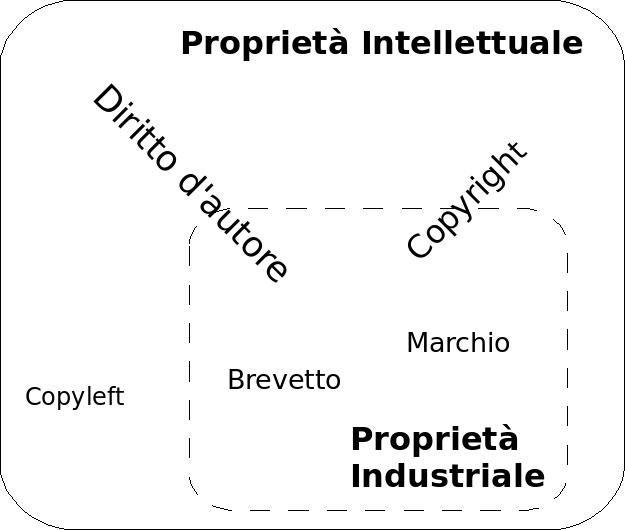
\includegraphics[scale=0.50]{figure/PI.png}
	\end{center}
	\caption{In figura è possibile notare la subordinazione del concetto di Proprietà Industriale a quella Intellettuale e l'intersezione o esclusione di concetti affini.}
\end{figure}



\section{Diritto d'autore e Copyright}
Si va riassumendo in questa sezione il diritto che si ottiene in maniera automatica con la creazione dell'opera, attraverso quella che precedentemente è stata definita come ``Proprietà Intellettuale''. Questa è una sostanziale differenza col brevetto che sarà discussa in \ref{sec:analogDiffBrevetti}.
Nelle scienze giuridiche il diritto d'autore è la posizione giuridica soggettiva dell'autore di un'opera dell'ingegno cui i diversi ordinamenti nazionali e diverse convenzioni internazionali, quale la Convenzione di Berna e la legge vigente, riconoscono la facoltà originaria esclusiva di diffusione e sfruttamento della stessa, ed in ogni caso il diritto ad essere indicato come tale anche quando abbia alienato le facoltà di sfruttamento economico.
Infatti come riporta \textit{l'art.25 della Legge 633/1941} dal diritto d'autore scaturiscono due facoltà che si riassuomo nei seguenti diritti:
\begin{itemize}
 \item Diritti Morali, non cedibili e mai cancellabili. Che si suddividono nei seguenti:

\begin{enumerate}
\item diritto alla paternità dell’opera
\item diritto all’integrit` dell’opera
\item diritto di inedito
\item diritto di ritiro dell’ opera per gravi ragioni morali, cio` il diritto di pentimento.
\end{enumerate}

 \item Diritti Patrimoniali o Economici, possono essere ceduti e terminano dopo il settantesimo anno dalla scomparsa dell'autore.
\end{itemize}


Scendendo nei dettagli, il diritto d'autore è una norma propria degli ordinamenti di \textit{Civil Law} come ad esempio l'Italia, laddove in quelli di \textit{Common Law} si parla di copyright, ad esempio negli gli Stati Uniti d'America.
Per quanto riguarda il copyright vi è da dire che giustamente nel gergo comune si utilizzano spesso indistintamente le espressioni copyright e diritto d’autore. I concetti infatti rimangono di una certà similarità se non per il diverso  sostrato social-economico in cui sono stati ideati.

Si può generalmente dire che il concetto di diritto d’autore è sostanzialmente più vasto del copyright: questo perchè
la matrice del copyright è di stampo anglo-americana, cioè dei cosidetti sistemi Common Law, ed è nato per tutelare l’industria culturale negli States. In questo senso è stato concepito in primis per tutelare l’interesse dell'accordo commerciale soggetto imprenditoriale/autore per la cessione di suddetti diritti.

Il diritto d’autore, partorito invece in Europa, fa un passo in più: l’attenzione della normativa si sposta verso la sfera dell’autore e non verso la sfera del commercio; in questo senso il diritto d’autore risulta più ampio del copyright, perchè aggiunge anche i cosidetti diritti morali incedibli.

Conludendo, poichè la trattazione è incentrata sulla tutela del diritto del software è importante sottolineare che ai diritti patrimoniali sul software sono state dedicate norme specifiche per quanto riguarda la legislazione italiana, ossia gli \textit{artt.64 bis, 64 ter e 64 quarter} della Legge 633/1941 che si conformano alla Direttiva 250/1991/CEE: i diritti esclusivi sui programmi per elaboratori (altresì chiamato \textit{software}) comprendono il diritto di effettuare e autorizzare:

\begin{itemize}
\item la riproduzione temporanea o permanente
\item la traduzione, l’adattamento
\item qualsiasi forma di distribuzione al pubblico compreso la locazione
\end{itemize}

Nonstante il diritto d'autore sia un concetto molto importante in luce anche alla trattazione delle licenza copyleft su cui si basa, si ritiene oppurtuno di dilungare la trattazione maggiormente sugli aspetti relativi alla ``Proprietà Industriale''. Per approfondire e capire maggiormente il concetto di copyright e del rapporto con la gestione dei diritti del software libero, denominata \textit{copyleft}, si consiglia la lettura di \cite[Simone Aliprandi - Teoria e Pratica del copyleft]{Aliprandi-copyleft2}.

Si continuerà quindi la tesi nel riportare i concetti di marchi registrato e brevetto; successivamente si vedrà come queste forme di tutela si applichino ai programmi per elaboratore e come intervenga la gestione alternativa dei diritti secondo license di tipo copyleft.\footnote{In particolare si approfondirà il caso della ricente licenza GPLv3 e delle diatribe collegate.}


\section{Marchi}
Dopo aver sintetizzato estremamente l'idea di base che sta dietro al diritto d'autore/copyright, si viene ad affrontare uno dei due interessanti concetti legati alla sfera della ``Proprietà Industriale''. In questa sezione infatti approfondiremo i marchi \textit{(trademarks)}.

Il trademark è definito come un segno distintivo ed indicativo creato da un individuo o da un impresa che identifica in maniera chiara un tipo di prodotto o servizio nella mente del consumatore: questa particolartà serve per discriminare il prodotto dagli altri. Il marchio è quindi un tipo di proprietà industriale sulla particolarità che mette in evidenza il prodotto/servizio: parole specifiche, nomi propri, disegni, loghi, cifre, suoni, confezioni e anche tonalità cromatiche. Quindi dopo aver registrato il trademark, si ha l'esclusiva commerciale di usare quel tipo di ``logo'' per identificare la propria impresa. Ovviamente questi vantaggi subentrano se le caratteristiche del marchio sono atte a distinguere i prodotti/servizi di un'impresa da quelli delle altre. Nei sistemi Common Law è possibile anche non registrare un marchio, ma conseguentemente sarà possibile solo proteggerlo nella aree geografiche dove viene usato e non oltre. Negli States inoltre quando ci si riferisce ad un marchio registrato che protegge un servizio, viene usato il termine \textit{service mark}.

Anche i marchi, così come i brevetti, trattati nella sezione \ref{sec:brevetti}, devono possedere dei requisiti per essere registrati. Questi requisiti sono riassunti nei seguenti punti:
\begin{description}
 \item[Requisito di novità] un marchio non è nuovo se simile o identico ad un marchio anteriore per prodotto/servizi identici o affini: e cioè per imprese che competono nello stesso mercato.
 \item[Requisito di originalità] il marchio deve essere atto a evidenziare o contraddistinguere il prodotto dell'impresa
 \item[Requisito di lecità] un marchio non deve essere contrario alla legge vigente o all'ordine pubblico e sociale.
 \item[Requisito di verità] un marchio deve trasmettere ai consumatori il vero ambito del prodotto/servizio. Non deve essere ingannevole nei loro confronti. 
 \end{description}

Superati questi requisiti ogni logo può seguire la procedura di refgistrazione secondo le leggi vigenti. C'è però un accordo globale che facilita la tutela internazinale dei trademarks.

Il principale accordo internazione per garantire e facilitare la registrazione di marchi in multiple legislazione risulta l'accordo/protocollo di Madrid. Esso costituisce un sistema centrale di amministrazione per una sicura registrazione dei trademarks estendendo la protezione di una \textit{registrazione internazionale} ottenuta tremie il WIPO \textit{(World Intellectual Property Organization)}. A questo protocollo aderiscono ben 71 stati di tutti il mondo.

La WIPO, in italiano Organizzazione Mondiale per la Proprietà Intellettuale, è una delle agenzie specializzate delle Nazioni Unite ed è stata creata nel 1967 con la finalità di incoraggiare l'attività creativa e promuovere la protezione della proprietà intellettuale nel mondo. Attualmente conta di 183 stati membri, regola 23 trattati internazionali ed ha sede a Ginevra, in Svizzera.

L'ultima accortezza da sottolineare è il sottilce cavillo che vi è tra marchio e designo comunitario. Infatti il disegno comunitario protegge i prodotti dell'industria del design a livello comunitario. Prima tale protezione era ristretta all'ambito nazionale, ma adesso quasi tutti i sistemi nazionali sono stati armonizzati e il design comunitario ha carattere unitario: esercita gli stessi effetti in tutti i paesi dell' Unione Europea presso l' UAMI (Ufficio per l'Armonizzazione nel Mercato Interno).

\subsection{Tipologie di Marchio}
Esistono vari tipi di marchio che possono essere registarti o no. Vengono spiegati nei punti seguenti:
\begin{itemize}
 \item Marchio di fatto. \`E un marchio non registrato che pur non essendo tale gode di una particolare tutela: chi ne ha fatto uso può continuare ad usarlo anche dopo la sua registrazione ottenuta da altri purché il suo uso sia confinato nei limiti territoriali e merceologici antecedenti la registrazione.
 \item Marchio forte/debole.
	\begin{itemize}
	 \item Un marchio forte è quello che ha spiccata originalità e notevole capacità distintiva (ad esempio non deve avere attinenza con il prodotto o servizio a cui si riferisce). Come ad esempio Ferrari (Auto) o Intel (Processori).
	\item Un marchio debole è, invece, quello che presenta una minore originalità (ad esempio per una diretta relazione con il prodotto o servizio che contraddistingue) pur mantenendo una minima capacità distintiva necessaria per differenziarlo ed essere tutelato. Come ad esempio vendita all'ingrosso o dettaglio di articoli sportivi.
	\end{itemize} 

\item Marchio di qualità. Esso ha la funzione di certificare che il prodotto sul quale è apposto abbia determinate caratteristiche qualitative e sia stato prodotto seguendo determinati procedimenti. Qui di seguito sono elencati i principali marchi di qualità:

	\begin{itemize}
	\item Marchio CE. Il Marchio CE attesta che il prodotto su cui è apposto è conforme a tutte le Direttive comunitarie ad esso applicabili.
	\item L'Unione Europea per promuovere e tutelare i prodotti agroalimentari ha creato con il Regolamento CEE n. 2081/92 i seguenti marchi: \textit{DOP} (Denominazione di Origine Protetta), \textit{IGP} (Indicazione Geografica Protetta) e \textit{STG} (Specialità Tradizionale Garantita).
	\end{itemize}

Questa categoria di marchi non deve essere registrata, ma la tutela deriva da apposite leggi introdotte dalla legislazione europea nel 1992 e molto simili ad alcuni sistemi già presenti in alcuni stati europei: in Italia dal 1963 è in vigore \textit{(DOC)} la Denominazione di Origine Controllata per i Vini.\footnote{Curiosità: l'Italia attualmente vanta il primato europeo tra i prodotti DOP, IGP e STG.}



\end{itemize}

\subsection{Marchi Registrati in Italia}
In questa parte si evidenza brevemente quello che costituisce il processo di registrazione di un marchio e i vari tipi di marchi contemplati in Italia.
La tutela di un marchio è disciplinata dagli art. 7 e seguenti del decreto legislativo n. 30 del 10 febbraio 2005: per essere tutelato giuridicamente un marchio deve essere registrato diventando così marchio registrato. La registrazione dura dieci anni a partire dalla data di deposito della domanda, salvo il caso di rinuncia del titolare e alla scadenza può essere rinnovata ogni volta per ulteriori dieci anni.
Essa deve effettuata presso l' UPICA (Ufficio Provinciale Industria Commercio e Artigianato) - sezione Ufficio Brevetti per Invenzioni, Modelli e Marchi - che si trovano presso le Camere di Commercio di ogni Provincia.
Comunque dopo la registrazione il marchio può decadere per le seguenti motivazioni:

\begin{enumerate}
\item  per volgarizzazione, cioè se il marchio sia divenuto nel commercio denominazione generica del prodotto o servizio oppure se abbia perduto la sua capacità distintiva;
\item per illiceità sopravvenuta cioè induca in inganno il pubblico  oppure sia contrario all'ordine pubblico.
\item per non uso, cioè se il titolare del marchio registrato non ne fa un uso effettivo entro cinque anni dalla registrazione o se ne sospende l'uso per un periodo ininterrotto di cinque anni, salvo che il mancato uso non sia giustificato da un motivo legittimo
\end{enumerate}

L'ultimo concetto da trattare a livello giuridico è si sintetizza con la parola  \textit{Licensing}: con questo termine il titolare del marchio concede ad un terzo il diritto di uso del marchio stesso. Di norma i contratti di licensing prevedono il diritto del licenziante di controllare la qualità dei prodotti sui quali il licenziatario appone il marchio.



\section{Brevetti} \label{sec:brevetti}
Il brevetto è lo strumento giuridico che conferisce all'autore di un'invenzione il monopolio temporaneo di sfruttamento dell'invenzione stessa, ossia il diritto di escludere terzi dall'attuare l'invenzione e dal trarne profitto. 

L'invenzione è la forma di protezione più forte che viene concessa a quei trovati che hanno un alto grado di innovazione, ma che, soprattutto, rappresentano una soluzione nuova ed originale ad un problema tecnico.

Il brevetto rappresenta pertanto un monopolio legale, se pur limitato territorialmente e temporalmente. Tale monopolio legale si giustifica con il fatto che il sistema brevettuale è basato su una forma di scambio: il titolare del brevetto riceve protezione per la propria invenzione e in cambio è obbligato a svelare e a descrivere l'invenzione. Le domande di brevetto e i brevetti già concessi sono infatti pubblicati dagli uffici brevetti di tutto il mondo e ciò li rende una primaria fonte di informazione tecnico-scientifica.

Possono costituire oggetto di brevetto i prodotti, i procedimenti produttivi, le varietà vegetali, mentre non sono brevettabili (art. 45 C.P.I.) ``le scoperte, le teorie scientifiche, i metodi matematici, i piani, i principi ed i metodi per attività intellettuale, per gioco o per attività commerciali, i programmi di elaboratori, le presentazioni di informazioni'' in quanto tali. 

Al di là della statica definizione legislativa riuscire a comprendere che cosa possa essere brevettabile come invenzione, richiede molto studio e molta pratica, anche se in modo sintetico si è soliti dire, con una definizione che soddisfa ben poco, che l'invenzione rappresenta una soluzione innovativa ad un problema tecnico; essendo solamente l'idea di fondo del sistema dei brevetti la stessa in tutti i paesi del mondo, si evidenziano profonde differenze nei vari sistemi brevettuali nazionali e continentali, che vanno non solo ad incidere nelle tecniche di brevettazione, ma discriminano anche nell'insieme delle tipologie di invenzioni brevettabili.

Lasciando l'analisi ancora in superficie rispetto alle casistiche particolari delle varie legislazioni, risulta importante chiarire secondo quali requisiti una invenzione è catalogabile come ``brevettabile'':
\begin{description}
 \item[Requisito di novità] L'oggetto del brevetto deve essere nuovo in modo assoluto, cioè non essere mai stato prodotto o brevettato in nessuna parte del mondo. Il concetto di novità viene inteso in senso ampio e si ricomprende nello "stato della tecnica" tutto ciò che è stato reso pubblico, in Italia o all’estero, prima della data di deposito della domanda di brevetto. Risulta chiarificatore un esempio banale per distinguere la brevettabilità dalla possibilità di produrre e/o sfruttare un invenzione: se un oggetto è stato realizzato o brevettato, ad esempio, in Cina ma non in Italia, ciò significa che chiunque in Italia potrà produrlo e venderlo, ma non certo che possa anche brevettarlo: la differenza è evidente, in quanto senza brevetto potrà agire in regime di libera concorrenza, senza pretendere di avere alcun monopolio.
\item [Requisito di originalità] Chiamato anche ``attività inventiva'' o ``non ovvietà'' sussiste ogni volta che l'invenzione non risulta in modo evidente dallo stato della tecnica per una persona esperta del ramo. Stabilire quando un trovato soddisfi questo requisito è estremamente difficoltoso in quanto è richiesto che l'invenzione per essere brevettabile non debba essere banale, ma rappresentare un progresso, un passo in avanti ``non ovvio'' rispetto allo stato della tecnica attuale. Proprio per stabilire quanto appena detto è spesso interessata la giurisprudenza, anche questa molto altalenante sui giudizi sull’argomento, ed è spesso intorno a questo punto che si giocano le cause relative alla nullità di un brevetto. 
\item [Requisito di industrialità]Risultano brevettabili solo soluzioni che possono essere riprodotte a livello industriale, escludendo tutte le applicazioni artigianali o comunque legate ad un contributo rilevante della persona che le ha realizzate.
\item [Requisito di liceità]Non sono brevettabili invece oggetti che possono ledere il senso del buon costume o essere contrarie all'ordine pubblico, concetti questi in continua evoluzione.
 \end{description}

Non da trascurare è l'aspetto legato ai diritti che poi scaturiscono dall'invenzione stessa; in seguito all'invenzione scaturiscono nei confronti dell'autore due tipologie diverse di diritto: il diritto morale sull'invenzione ed il diritto di brevetto. Mentre il primo concerne un'area strettamente personale e non è cedibile, il secondo riguarda lo sfruttamento economico dell'invenzione, e quindi risulta cedibile.
% 	\subsection{Royalties}
\subsection{Il brevetto in Italia}
Nello stato italiano la normativa sui brevetti è stabilita dal Titolo IX del Libro Quinto del Codice Civile, intitolato ``Dei diritti sulle opere dell'ingegno e sulle invenzioni industriali''. 

Nel dettaglio l'articolo specifico è il 2585, che definisce l'oggetto del brevetto come segue:

\textit{``Possono costituire oggetto di brevetto le nuove invenzioni atte ad avere un'applicazione industriale, quali un metodo o un processo di lavorazione industriale, una macchina, uno strumento, un utensile o un dispositivo meccanico, un prodotto o un risultato industriale e l'applicazione tecnica di un principio scientifico, purché essa dia immediati risultati industriali.''}

Rimane da precisare che in Italia tutta la materia gravitante attorno al campo della Proprietà Intelletuale e Brevetti è regolamentata da una apposita legislazione, confluita dal 2005 (con la legislazione sui marchi, modelli, design registrati) nel D.Lgs. 10 Febbraio 2005, chiamato codice della Proprietà Intellettuale.

Riguardo alla brevettabilità non è possibile, per la legislazione italiana, registrare un indice di ciò che è catalogabile come ``brevettabile''; si ritiene comunque che la serie di requisiti richiesti sia sostanzialmente analoga a quella anticipata nella sezione precedente, come possiamo evincere dagli articoli 46 e 48 del Codice della Proprietà Intellettuale. 

Tuttavia sono note e tassative la categorie di eccezioni, ovvero le aree di lavoro e di scoperta non brevettabili. Queste comprendono:
\begin{itemize}
\item le scoperte, le teorie scientifiche e i metodi matematici
\item i piani, i principi e i metodi per attività intellettuali, per gioco o per attività commerciali e i programmi di elaboratori;
\item le presentazioni di informazioni
\item i metodi per il trattamento chirurgico o terapeutico del corpo umano o animale e i metodi di diagnosi applicati al corpo umano o animale; possono però esserlo i prodotti, in particolare sostanze o miscele di sostanze, impiegati per l'attuazione dei metodi diagnostici, terapeutici o chirurgici: non costituisce invenzione il metodo, possono costituirla gli strumenti necessari alla sua applicazione.
\item le razze animali, eccezione fatta per i procedimenti microbiologici\end{itemize}

L'autore dell'invenzione ha il diritto di disporre della stessa e di commericalizzarla. Questi diritti sono intesi come diritti patrimoniali, e sono riconosciuti come propri dell'inventore; l'aggettivo ``patrimoniali'' sottolinea la classe di diritti che possono essere oggetto di cessione, solitamente mediante contratto e a titolo oneroso.

Come già avevamo accennato nella trattazione generale esiste anche nella legislazione italiana il riconoscimento per il diritto morale, che risulta incedibile, intrasmissibile e strettamente personale. 

L'autore dell'invenzione deve richiedere la registrazione del brevetto presso l'ufficio italiano brevetti, che è responsabile della verifica dei requisiti sopracitati e della non contrarietà alle leggi; se tutto è ritenuto regolare si procede alla registrazione del brevetto.

Normalmente la durata della tutela brevettuale è ventennale, ma esistono delle clausole che possono indurre una prescrizione anteriore; se ad esempio il titolare del brevetto non lo rinnova, oppure se entro tre anni dalla registrazione del brevetto l'invenzione non è ancora conclusa. Esistono anche uteriori casistiche, indotte dalla dipendenza di ulteriori brevetti o dalla situazione di inventori dipendenti subordinati di aziende, ma non essendo strettamente inerenti alla trattazione saranno trascurate.

L'azione spettante a chi viola un brevetto industriale è quella di contraffazione.

\subsection{Il brevetto nell'Unione Europea}
Il Brevetto Europeo è una tutela Istituita con la Convenzione di Monaco sul brevetto europeo del 1973, riprendendo le indicazioni della Convenzione di Strasburgo del 1963. 

L'ente responsabile della brevettazione a livello comunitario è l'``Organizzazione europea dei Brevetti'' (in lingua inglese, \textit{European Patent Organisation}, da cui deriva l'acronimo EPO) è un'organizzazione pubblica internazionale creata dalla Convenzione europea dei Brevetti. L'Organizzazione europea dei Brevetti ha sede a Monaco di Baviera, in Germania.
\begin{figure}[hb]
\centering
	
\includegraphics[scale=0.8]{epo.png}
\caption{\textit{Il logo dell'European Patent Organisation}}
\end{figure}
Il brevetto europeo non esiste però come entità unitaria; il nome che porta ha in se' una valenza unitaria che rappresenta la validità del brevetto all'interno dell'Unione Europea, ma non come documento unitario, bensì come collezione di brevetti nazionali che conferiscono all'inventore i diritti che conferirebbe l'ottenimento di ogni singolo brevetto nazionale.  

I brevetti europei sono concessi dopo un'accurata ricerca dello stato della tecnica ed un esame di merito che ne verifica i requisiti di brevettabilità.
\subsection{Il brevetto Internazionale}
Rispecchiando la procedura comunitaria, a livello internazionale è stato redatto un trattato, gestito dall'Organizzazione Mondiale della Proprietà Intellettuale (OMPI, più nota con l'acronimo internazionale WIPO \textit{World Intellectual Property Organization}): il PCT (Trattato di Cooperazione in materia di Brevetti).
\begin{figure}[hb]
\centering
	
\includegraphics[scale=0.4]{wipo.png}
\caption{\textit{Il logo del World Intellectual Property Organization}}
\end{figure}
Quest trattato nasce con lo scopo di offrire una procedura unica per ottenere un brevetto simultaneamente in un grande numero di paesi, anch'esso senza l'introduzione di una certificazione unica sovranazionale. L'Italia vi aderisce dal 1985.

La procedura stabilita dal PCT innesca la stessa serie di procedure previste negli stati designati, unificando e facilitando la messa in moto della macchina brevettuale, tramite un'unica domanda.

Ogni richiesta è oggetto di una ricerca internazionale effettuata da un ufficio brevetti incaricato, che la svolge per conto dell'OMPI; nel caso dell'Italia l'ufficio competente è l'Ufficio Europeo dei brevetti. Il risultato della ricerca è pubblicato in un rapporto di ricerca internazionale che riporta la lista dei documenti che potrebbero attaccare la brevettabilità del contenuto della domanda.

La procedura PCT offre anche la possibilità di richiedere un esame internazionale preliminare da parte dell'autorità incaricata, ottenendone un parere sulla brevettabilità dell'oggetto delle rivendicazioni. Tale parere può dare maggiori informazioni sull'opportunità di continuare la procedura con buone possibilità di successo, ma esso non è vincolante per gli uffici nazionali che, indipendentemente, dovranno decidere sul rilascio del brevetto.

\section{Analogie e Differenze}\label{sec:analogDiffBrevetti}
%Questa sezione piu che lunga deve essere efficace e sintetica. magari con una tabellina

Si viene ora all'ultima parte di questo capitolo in cui si vuole riassumere i concetti espressi su diritto d'autore, brevetti e marchi. In particolare si riesce a trattere le profonde differenze che sussiste tra copyright vs. brevetto/marchio, ma si capisce anche come mai il brevetto industriale ha bisogno del copyright per essere attuato giustamente.

In questo senso il brevetto in qualche modo dipende dal diritto d'autore e quindi appartiene alla tutela della Properità Intellettuale perchè è l'inventore che detiene il diritto di essere riconosciuto come autore e in maniera conseguenziale detiene anche il diritto al brevetto. Quindi in questo senso si può dedurre una dipendenza tra i due o quanto meno un collegamento.\\
Il brevetto però prosegue oltre entrando nel campo della Properità Industriale: in questo senso si hanno altri diritti che devono essere registrati in maniera formale, al contrario del copyright. Questa registrazione dà la facoltatà allo sfruttamento dell'invenzione in regime di monopolio temporaneo, cosa che il copyright non prevede.

\begin{tabular}{l|l|l|l}
	~ & \textbf{Copyright} & \textbf{Brevetto} & \textbf{Marchio} \\ \hline
	\textbf{Registrazione} & No & Sì & Sì \\ \hline
	\textbf{Tutela} & x & x & x\\ \hline
	\textbf{Proprietà} & Intellettuale & Industriale & Industriale \\ \hline
	\textbf{Monopolio} & No & Sì & Sì
\end{tabular}



\chapter{La proprietà intellettuale in campo software}
Dopo aver delineato la sfera della Proprietà Industriale e Intellettuale, si cerca di fare luce sull'attuale sistema di tutela dei diritti che si acquisicono con la scrittura di un programma per elaboratori; si cerca di cogliere in esso la giusta forma di tutela,  confrontando in particolare realtà diverse della forma di tutela del brevetto in UE e in USA.

\section{Il sistema giuridico delle licenze} \label{sec:sistema-licenze}
Attualmente il software è concepito come espressione dell'intelletto umano, cioè opera dell'ingegno a carattere creativo, e ovviamente ricade nella tutela della Proprietà Intellettuale. Per questo chiunque scrive un programma per elaboratore detiene il così detto copyright, cioè tutti i diritti che si sono evidenziati nel capitolo \ref{cap:uno}.

Si vedrà successivamente come in alcuni casi il diritto d'autore verrà scavalcato dal brevetto nella casistica di brevettazione di un processo fisico che viene associato ad un programma software. \`E stata infatti questa la pratica di molte aziende per iniziare a brevettare il software in via alternativa. Questo aspetto però sarà trattato nelle sezioni sucessive, dove si farà luce sulla storia della brevettazione software in UE e in USA.

Principalmente il software è prodotto con enormi investimenti per uno scopo molto semplice: l'uso. Negli anni '80 e '90, le software house hanno lucrato su questa rivoluzione digitale fino a diventare multinazionali o comunque colossi dell'informatica.

Si è cercato fin da subito quindi di tutelare il software in maniera tale da avere la possiblità di venderlo, pur rimanendo sempre i proprietari. Come si sa su di esso si possiede il diritto d'autore (cioè la proprietà intellettuale, non la proprietà del supporto con cui viene venduto) ed è proprio su questa facoltà che è nato il contratto tra un licenziatario \footnote{colui che ne detiene il copyright e ne cede alcuni in cambio di denaro o altro} e un licenziante \footnote{qualsiasi utente dell'opera}. Questo accordo scritto prende comunemente il nome di licenza.

Nel particolare la licenza segue il modello uno a molti tra licenziante e licenziatario e si definisce con il termine ``contratto di licenza''. La parola contratto deriva dal modo di tutelare la trasmissione dei diritti d'autore cioè nel senso classico di accordo  tra due o più parti per costituire, regolare o estinguere un rapporto giuridico patrimoniale”.
Il termine licenza invece si definisce come un atto unilaterale giuridico, originario del diritto amministrativo, con cui un soggetto concede un' autorizzazione a compiere una determinata attività. \`E importante sottolineare come l'uso del vocabolo ``licenza'' derivi dal termine coniato negli States e tradotto letteramente da \textit{mass market licenses of copyright material }.

In sintesi quindi l'obietto che si prefigge una licenza riguarda cessione di alcuni diritti come, ad esempio, il diritto all'uso: infatti con l'acquisto di un software, e la conseguente sottoscrittura alla licenza, non si compra il software in sè, inalienabile dall'autore, ma il diritto all'uso e in alcuni casi (come nel copyleft) anche il diritto alla modifica e alla copia/ridistribuzione.

In questa sezione si è visto come inizialmente in tutte le legislazione l'idea di software coincida con un' opera logico-matematica tutelabile da diritto d'autore e quindi appartenente alla sfera della Proprietà Intellettuale. Ovviamente poi si è reso necessario una forma più stringente e tagliente di tutela che in qualche modo poteva tutelare le lobby del software anche dalla possibile minaccia di copia tra sè stesse, visti la particolare natura immateriale/virtuale del software e il boom industriale legato al suo commercio.

Questo atteggiamento è ampiamente attecchito ``de facto'' in America e invece meno ratificato in Europa in quanto il dibattito risulta ancora acceso anche da un punto di vista politico.

\section{La situazione dell'UE sui brevetti software}
La situazione europea e mondiale sulla questione dei brevetti software è molto spinosa, in quanto risulta molto complesso delimitare i confini per cui il software inteso come esclusivo codice possa ritenersi brevettabile oppure una invenzione tecnica basata su software possa ritenersi non brevettabile.

Nell'Unione Europea l'Organizzazione Europea dei Brevetti ha rilasciato molti brevetti su invenzioni basate almeno in parte su software da quando è in vigore, dagli anni '70, la Convenzione europea dei Brevetti, nonostante proprio in Europa, per la precisione in Francia nel 1968\cite{invenzione-software}, sia nata la prima norma in materia brevettuale tesa ad escludere dalla tutela i programmi per elaboratore.

L'articolo 52  della convenzione esclude esplicitamente i programmi per computer dalla brevettabilità (comma 2), intesi come programmi per computer in quanto tali (comma 3). L'interpretazione data all'articolo è che ogni invenzione che offre un contributo tecnico non ovvio o risolve problemi tecnici in maniera non banale sia brevettabile anche se comprende una parte software.

Ovviamente non può essere sufficiente affidare l'intera legislazione di un settore così importante a livello scientifico ed economico ad una mera distinzione di carattere semantico, ma deve essere approfondito l'ambito di utilizzo e di realizzazione del software stesso.

Prima di tutto è da notare che è impossibile che il legislatore abbia impiegato la definizione ``programmi in quanto tali'' riferendosi esclusivamente alla forma codificata delle informazioni, lasciando brevettabili tutti i processi che le istruzioni producono, in quanto il software è stato incluso nella categria delle opere non brevettabili come ``attività intellettuale'' e non come ``presentazione di informazioni''.

Per inquadrare correttamente il software all'interno della disciplina brevettuale occorre prenderlo in considerazione in due momenti: innanzitutto come registrato su un supporto di memorizzazione (inteso quindi come insieme di informazioni, sequenza di istruzioni), in secondo luogo all'atto dell'esecuzione, quando tramite le istruzioni va a regolare il comportamento della macchina.

Il primo momento dei due appena descritti è stabilmente appartenente all'area del non-brevettabile, essendo il funzionamento del supporto completamente indipendente da ciò che ne viene memorizzato sopra, ed essendo totalmente libero il genere di informazioni che possono essere registrate sul supporto. Ristretto a questo momento il concetto di software è riconducibile alle ``presentazioni di informazioni'', escluse dalla brevettabilità con chiarezza (articoli 52 n.2 lett.\textit{d} CBE e 12 co.2 lett.\textit{c} l.i.).

Il momento di interesse alla trattazione è quello che riguarda il funzionamento del software all'interno dell'elaboratore, in quanto si realizza lo scopo pratico per cui il software è stato scritto.

La tesi che supporta la non brevettabilità del software appoggiandosi alla separazione fisica tra software ed hardware, attribuisce totale indipendenza alla funzionalità del software in riferimento allo specifico hardware su cui viene eseguito. Una procedura, idealmente, può essere eseguita su qualsiasi tipo di computer implicando quindi che lo sforzo mentale che ha portato all'invenzione della procedura prescinda dalla macchina sulla quale poi sarà implementata.

L'hardware non può essere quindi considerato come parte integrante dell'invenzione; la presenza di questo nell'esecuzione del software (nonostante sia composto da tutti componenti brevettabili) non è sufficiente a sancire la brevettabilità del software.

Esiste anche una ricostruzione più rigida, sempre a favore della non-brevettabilità del software e di matrice più dogmatico/filosofica, nata in Germania prima che il paese si adattsse alla convenzione di Monaco. In questa ricostruzione l'attenzione è spostata a livello ``ontologico'' sulla differenza che intercorre tra il concetto di ``invenzione brevettabile'' e ``algoritmo''. \`E da precisare che, nonostante questa interpretazione ormai superata dalla convenzione di Monaco a livello temporale, è tuttora ritenuta il fondamento della non brevettabilità del software in Europa, e viene citata come fonte ideologica di questa scelta.

In Germania è ormai una definizione classica di ``invenzione brevettabile'' un qualcosa che insegni ad utilizzare le forze naturali, fatto eccetto di quelle che regolano l'attività mentale, con il fine di ottenere un nuovo risultato tangibile direttamente attraverso il dominio dei rapporti causali relativi a tali forze.

L'algoritmo invece è concepito come una procedura astratta per la soluzione di un problema, la cui validità e risultato prescindono dall'impiego diretto delle forze della natura; l'uso di mezzi materiali è quindi successivo al completamento dell'idea inventiva, in quanto riguarda solamente una sua possibile attuazione.

Per cui emerge da questa teoria che il problema di carattere tecnico riguardante la realizzazione dell'hardware in grado di svolgere le operazioni richieste dal software è indiscutibilmente appartenente alla categoria del ``brevettabile'' mentre il problema concernente la procedura logico-matematica che poi dovrà essere attuata meccanicamente dalla macchina si risolve prima di entrare nella sfera del mondo fisico, in quanto i risultati sono costanti e ripetibili indipendentemente, e possono essere dimostrati anche su un piano meramente astratto.

Su questa base, l'attività del programmatore di tradurre (successivamente alla concezione logica della procedura) l'algoritmo in un concreto software non aggiunge niente al concetto espresso dall'invenzione dell'algoritmo; è come se il programmatore eseguisse un'attività compilativa, all'interno di confini già tracciati dall'invenzione della procedura algoritmica. La stesura del software quindi si concentra nello sfruttare la macchina secondo il suo scopo.

La conclusione di questo pensiero porta quindi a evidenziare che nell'invenzione di software è assente l'utilizzo diretto delle forze della natura, in quanto l'impiego dei mezzi fisici non è collegato causalmente all'attività inventiva. I mezzi fisici intervengono solamente al termine del processo inventivo, ovvero al momento della trasofrmazione dell'algoritmo in programma, confermando pertanto la non brevettabilità di questo.

All'interno dell'Unione Europea finora è riuscito a rimanere saldo questo principio, riconosciuto anche dal Parlamento Europeo stesso in più momenti. Il più importante di questi è stato probabilmente il 24 settembre 2003, dove è stata riconosciuta la separazione del software dal contesto tecnico e ne è stata limitata la brevettabilità; l'atto tecnico è stata l'approvazione in prima lettura della Direttiva Europea n.2002/47 con l'apporto (rispetto al provvedimento originario del 2002) di numerosi e fondamentali emendamenti che confermano il divieto di brevettazione del software .

Nonostante la pressione di molte \textit{lobby} del settore informatico, che hanno indotto il Consiglio dell'Unione Europea in primis (18 maggio 2004) e la Presidenza dell'Unione Europea in seconda battuta (7 marzo 2005) a tentare di ribaltare, tramite una direttiva, la decisione parlamentare a favore della non brevettazione del software, il 6 luglio 2005 con 648 voti favorevoli, 14 contrari e 18 astenuti, il Parlamento Europeo ha ripristinato quanto legiferato nel 2003, bocciando in seconda lettura tale direttiva e riconscendo la non brevettabilità del software all'interno dell'Unione Europea.

\section{I brevetti software in USA}

Molto diversa e più ben decisa nelle scelte (almeno apparentemente) dalla situazione europea, appare la gestione dei brevetti software negli Stati Uniti. Questa è da mettere in luce in quanto è il paese che detiene, secondo i dati forniti dal USA Paten Office, circa il 60\% del mercato mondiale del software.

Innanzitutto anche negli States si ebbe l'echeggiare della prima interpretazione data alla brevettabilità del software: la concezione tedesca dell'assenza di carattere tecnico dei programmi, considerandoli alla stregua di \textit{mental steps} non brevettabili. Questa concezione incontrò infatti nei primi anni '60 l'appoggio del Patent Office. Questo orientamento però incontrò tuttavia una radicale opposizione da parte della giurisprudenza della \textit{Court of Costum and Patent Appeal}, fintantochè non si arrivò negli anni '70 a non considerare più programmi per elaboratori come meri algoritmi matematici.

Più nel dettaglio il caso più emblematico di questa concezione derivante dalla Germania, fu il primo caso in cui il problema della brevettabilità del software venne esaminato: fu il caso denominato ``Gottschalk v. Benson'' in cui, nel 1972, la Corte Suprema si occupò della possibilità di brevettare un programma per elaboratore consistente in un metodo di conversione di un sistema decimale codificato in binario in un sistema binario puro mediante l'uso di un algoritmo. La conversione poteva essere effettuata anche a mano, ma l'algoritmo consentiva di farla effettuare ad un elaboratore in modo da risparmiare tempo ed energie. La Corte Suprema si affermò contraria alla brevettabilità del richiesto algoritmo ritenendo il processo di conversione sopra citato un vero e proprio algoritmo, ossia una procedura per la soluzione di un problema matematico che, in quanto tale, non è brevettabile. Ciò per evitare il crearsi di un diritto di monopolio su una formula matematica, su un concetto o su un modo di pensare che devono essere lasciati al libero sfruttamento di chiunque e che, per definizione, non poteva essere messo sotto brevetto.

Mentre le richieste di brevetto pervenivano sempre più numerose, la prima decisione con la quale la Corte Suprema sanzionò la validità di un brevetto concernente un programma per elaboratore, fu con il successivo e fondamentale caso denominato ``Diamond v. Diehr'' del 1981. In questo caso la Corte Suprema stabilì che l'ufficio brevetti doveva concedere un brevetto, anche se una parte importante dell'invenzione consisteva in un programma per elaboratori che utilizzava formule già note: la Corte Suprema affermò che in questo caso l'invenzione non era un mero algoritmo matematico, ma un processo per fondere la gomma, quindi brevettabile. Tecnicamente si brevettava un software utilizzato nel processo di stampaggio degli oggetti di gomma che consentiva di controllare ripetutamente la temperatura all'interno dello stampo e calcolare il tempo ottimale di formatura, trascorso il quale il programma comandava l'apertura dello stampo medesimo.

In seguito e questo evento furono concessi altri brevetti su software anche se con risultati contrastanti e confusi. Questo perchè inizò a decadere quella valenza logico matematica che aveva caratterizzato negli anni 50-60 l'Ufficio Brevetti. In particolare ``mental step doctrine'' cadde per i seguenti motivi:

\begin{itemize}
	\item si distinse tra processi/passi mentali e steps eseguiti meccanicamente da un disposivo fisico come un calcolare.
	\item si differenziò l'indeterminatezza della logica umana dalla determinatezza delle macchina
	\item Si osservò che una dispositivo fisico è composto da hardware e software e che questo'ultimo può cambiare il comportamento del dispositivo fisico
\end{itemize}
In questo senso queste obiezioni misero in luce gli aspetti che distinguono i programmi per elaboratore dalle creazioni tradizionali escluse dalla brevettazione, mettendo sempre pià in evidenza una sostanziale unione tra hardware e software, contrariamente al dibattito del'Europa e  diversamente dalla visione tedesca in cui il software si riduce all'esecuzione, secondo modalità prestabilite, di una procedura in sè già completa indipendentemente dai mezzi in cui è svolta.

In USA poi la Corte d'Appello del Circuito Federale tolse ogni dubbio attraverso una serie di regolamentazioni che inquadravano il software eseguito su una macchina come un dispositivo fisico. La prima denominata \textit{In re Alappat} afferma che un nuovo algoritmo abbinato ad un'elementare componente fisica costituisce un nuovo dispositivo fisico. Ne consegue che un calcolatore su cui è caricato un algoritmo originale diventa una ``nuova macchina'', brevettabile secondo le tradizionali normative statunitensi sul software. Ciò venne ulteriormente sostenuta da una seconda norma \textit{In re Lowry} che affermava che le strutture di dati rappresentanti l'informazione contenute in un disco fisso o una memoria deve essere similmente considerata come un dispositivo fisico.

In conclusione negli anni '90 ci fu la svolta definitiva a favore dei brevetti: attraverso la nomina di Bruce Lehman commissario dell'ufficio brevetti e marchi, il quale non era un avvocato specializzato in brevetti ma uno dei principali lobbisti dell'industria del software; nel 1995 l'ufficio stabilì alcune linee guida per l'esame e la registrazione di brevetti software, diventando così senza una piena decisione, apparentemente validi.

In sintesi dalla travagliata storia Americana, è pacifico ormai che non si possa escludere la brevettabilità un processo solo perché si contiene un software;e d'altro canto, non è sufficiente dire che l'invenzione si sostanzia in un algoritmo per rigettare la domanda di brevetto. Ancora, non è vero che un'invenzione non può essere brevettata perché il procedimento è eseguito da un elaboratore e è descritta sotto forma di un programma elettronico. Vista la sostanziale affinità tra algoritmi matematici e software, sarà ritenuto brevettabile quel software che non si esaurisca in alcuna formula o algoritmo matematico, ma si concretizzi, al contrario, in un'applicazione pratica.

Su qeusta linea si è messo a punto un criterio basato su un duplice accertamento \textit{(two steps doctrine)} per poter distinguere i programmi brevettabili da quelli non brevettabili. Per quanto riguarda il primo accertamento la Corte \textit{(Court of Customs and Patent Appeals)} afferma che occorre distinguere tra un concetto di algoritmo più ampio ed uno più ristretto. Il primo comprende quei procedimenti in cui la successione delle attività necessarie per realizzare un determinato fine è descritta passo dopo passo \footnote{a step-by-step procedure for solving a problem or accomplishing some end}; il secondo comprende soltanto quei procedimenti volti a risolvere un problema matematico.




\begin{figure}[bh]
	\begin{center}
		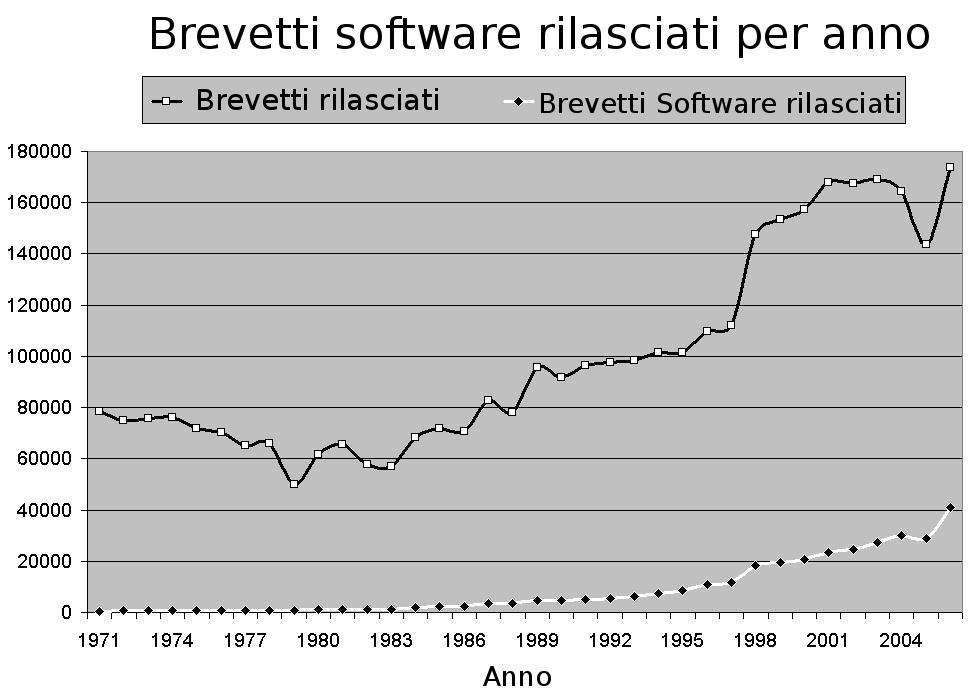
\includegraphics[scale=0.55]{figure/UsPatent.png}
	\end{center}
	\caption{\textit{Nel grafico è possibile notare la cresciata dei brevetti rispetto a quelli software nel mercato USA}}
\end{figure}


 \chapter{Il software libero nel sistema giuridico informatico}

Appurate le definizioni di forma di tutela della Proprietà Intellettuale come copyright, brevetto e marchio nel capitolo 1 e la storia dei brevetti applicati software nei mercati più sviluppati come USA e UE nel capitolo 2, si sfrutta i seguenti due capitolo dell'elaborato per approfondire il dibattito sulla tutela del software che oscilla tra copyrigt e brevetti.

In particolare nel capitlo 3 si approfondirà come il movimento opensource stia cercando di difendersi dalla brevettazione del software attraverso la licenza madre copyleft \textit{par excellence}: la GPL, modificata di recente per questo motivo approdando alla terza versione.
In questo trattato non si approfondiranno nè i concetti di opensource o free software nè il concetto di copyleft, che invece possono essere conosciuti rispettivamente attraverso la lettura di \cite[Compendio di libertà informatica e cultura open]{Aliprandi-compendio} e \cite[Copyleft e Opencontent]{Aliprandi-copyleft}

Il capitolo 4 invece sarà più pratico: si metteranno in luce delle conseguenze che la brevettazione software apporta sia nel software libero che in quello proprietario e commerciale; quindi si farà un esempio di brevetto, verrà spiegato e si vedrà le conseguenze portati in USA e in UE.

Adesso si va ad approfondire alla luce di quanto visto fino ad ora, come si tutela il \textit{free software} nel sistema giuridico informatico.


\section{Le licenze libere}
Breve introduzione
	\subsection{La licenza GPL}
	breve
\section{L'approccio ai brevetti della nuova licenza GPLv3}
va letta la GPL3 e spulciata per quanto riguarda i brevetti riportando magari qualche tratto saliente.
\section{Un esempio di brevetto vincolato dalla GPLv3}
idem


\chapter{Un esempio concreto: il caso MP3}
Per rendere chiara e comprensibile la trattazione sarà portata come esemplificativa uno delle questioni più famose e rilevanti nella storia della brevettazione software, sia per l'importanza dell'invenzione sotto brevetto, sia per la rilevanza economica che ha avuto la causa giudiziaria di violazione di brevetto che ha colpito una delle più importanti aziende informatiche: Microsoft Corporation.

Rilevante sarà anche l'analisi del comportamento che deve essere tenuto nelle varie regioni mondiali in virtù della valenza o meno del suddetto brevetto: per chiarire questa problematica sarà portato come esemplare il comportamento della distribuzione GNU/Linux più diffusa al momento, Ubuntu Linux\cite{ubuntu}.

\section{Cos'è l'algoritmo di compressione MP3}
La discussione di questo capitolo verte su uno degli algoritmi più importanti della storia informatica degli ultimi tempi: l'algoritmo di compressione audio \textit{MPEG-1/2 Audio Layer 3}, comunemente noto come MP3. Questo algoritmo di compressione è diventato noto per la sua capacità di ridurre drasticamente la quantità di dati richiesti per la riproduzione di un suono, mantenendo comunque una riproduzione fedele del suono originario. Nei moderni codificatori MP3 gli algoritmi più efficaci fanno di tutto per assicurare che i suoni rimossi siano quelli che non possono essere rilevati dall'orecchio umano. Questo risultato è stato ottenuto anche grazie alla scienza della psicoacustica.

Nonostante ne siano stati riconosciuti molti difetti, diversi dei quali superati anche da algoritmi successivi ed alternativi (si pensi all'algoritmo \textit{AAC MPEG-4} oppure all'\textit{Ogg Vorbis}) il formato .mp3 (classico dei files compressi con tale algoritmo) risulta ancora il più diffuso in campo musicale, e ciò spiega la portata economica che può comportare l'eventuale copertura brevettuale sull'invenzione.
\section{Il brevetto sull'MP3}\label{mp3-patent}
La Thomson Consumer Electronics è la proprietaria principale del brevetto di MPEG-1/2 Layer 3 in U.S.A. e Giappone, e ha raccolto in un apposito sito (\textit{http://www.mp3licensing.com/}) tutte i brevetti relativi all'MP3 che detiene (svariati validi anche in UE), e una riepilogativa tabella delle royalties che le aziende devono pagare per utilizzare codificatori e decodificatori di MP3.
\begin{figure}[hb]
	\begin{center}
		
\includegraphics[scale=0.75]{figure/mp3.jpg}
	\end{center}
	\caption{\textit{Il logo del sito Thomson sui brevetti MP3}}
\end{figure}
\subsection{Ricerca del brevetto}

\subsection{Termini del brevetto}

\subsection{Aree di valenza e royalties}

\section{Il delicato rapporto tra Microsoft ed il formato MP3}
Scendendo nelle notizie di attualità è comune trovare, in campo tecnico/ingegneristico, notizie di violazioni di brevetto, di violazione di proprietà intellettuali e simili. Un po' meno raro è trovare eventi che vedano implicati i brevetti software, specialmente in Europa, dove, come abbiamo visto, sono quasi impossibili da ottenere. 

\`E normale quindi che faccia scalpore quando un tribunale emette una sentenza di violazione di brevetto informatico contro una azienda; è ancora più normale che l'interesse salga a livelli inauditi se l'azienda coinvolta è la più fiorente in campo informatico, e viene condannata ad una pena pecuniaria pari al fatturato di una decina di anni di una azienda normale. Stiamo parlando della Microsoft, e della \textit{querelle} giudiziaria che l'ha vista protagonista con Alcatel-Lucent.

La questione è spinosa in quanto non vede solo motivazioni giuridiche tra i proprietari originari del brevetto ed il presunto violatore, ma vede di fronte al presunto violatore delle enormi aziende che hanno inglobato in percentuali diverse le originali proprietarie del brevetto, lasciando innescare quindi procedure economico/giudiziarie dalla portata enorme.

Nel caso di MP3, come è stato detto nella sezione \ref{mp3-patent}, il principale detentore della proprietà brevettuale è Thomson Consumer Electronics, ma non è affatto ne' l'unica ne' l'originaria proprietaria. Gli algoritmi di base di MP3 sono stati sviluppati originariamente in collaborazione tra il Fraunhofer Institute e gli ex-Bell Laboratories. Il primo gruppo a rilasciare un encoder fu il Fraunhofer Institute nel 1994, e Microsoft ha sempre sostenuto di aver ottenuto in licenza la tecnologia proprio da quest'ultimo, pagandola ben 16 milioni di dollari ed integrandola nei sistemi operativi Windows attraverso i codec e il lettore software Windows Media Player.

Thomson è di fatto la società che al momento controlla il Fraunhofer Institute, mentre Alcatel-Lucent al momento detiene la proprietà dei Bell Laboratories.

Proprio Alcatel-Lucent nel 2003 ha trascinato in tribunale i produttori di PC Dell e Gateway per l'utilizzo illegittimo dei suoi brevetti. Microsoft, in accordo con i patti di indennizzo stretti con le due società, ha offerto loro protezione legale ed ha ottenuto come contropartita la denuncia di Alcatel per la violazione degli accordi di sfruttamento dei brevetti sulla console Xbox 360. Le due aziende avevano stretto un'intesa sulla prima Xbox ma Alcatel-Lucent ha sostenuto davanti al giudice - e ha infine ottenuto una sentenza a proprio favore - che l'accordo non comprendeva la nuova versione; in tutto la disputa riguardava ben quindici violazioni di brevetto, e dopo il rigetto delle prime due accuse, nel Febbraio del 2007 è arrivata la notizia di una sconfitta giuridica per la Microsoft, per la violazione appunto del brevetto riguardante MP3. La sanzione prevedeva una multa per più di un miliardo e mezzo di dollari, valutati i benefici sfruttati abusivamente da Microsoft nel proprio sistema, valutata la diffusione del formato MP3 e la diffusione del sistema Microsoft stesso.

Il motivo principale della diatriba è strettamente legato alle royalties\footnote{Con il termine royalty si indica il pagamento di un compenso al titolare di un brevetto o una proprietà intellettuale, con lo scopo di poter sfruttare quel bene per fini commerciali.} che le aziende devono pagare per poter utilizzare il formato MP3. Come si può vedere nell'elenco pubblico disponibile nel sito Thomson già citato in precedenza, Microsoft risulta considerata tra le aziende autorizzate all'utilizzo della tecnologia; Alcatel, cercando di sfruttare altri processi già aperti contro la casa di Redmond ha tentato di avvalersi del presunto diritto di riscuotere ulteriori royalties sul formato, in virtù dell'acquisizione dei Bell Laboratories.

La questione, ancora non definitivamente sciolta in quanto è ancora possibile un ulteriore grado di giudizio, ha visto la sentenza in appello ribaltare, e di fatto annullare, la sentenza contro Microsoft, riconoscendo sufficiente il pagamento del brevetto presso uno dei proprietari legittimi.

Non ha comunque avuto vita facile la casa di Redmond verso questo formato di compressione audio. Mentre negli Stati Uniti, dove vige il brevetto, ha dovuto sostenere questo lungo processo (non ancora terminato), risulta interessante vedere anche il trattamento che le è stato riservato nell'Unione Europea, dove i brevetti principali dell'MP3 non sono validi.

La Microsoft, dovendo produrre un sistema operativo con bacino d'utenza mondiale, ha inizialmente provato a ``boicottare'' questo formato, cercando di far abituare i suoi utenti al suo formato proprietario (.wma) senza fornire il proprio sistema operativo del supporto per MP3. Questo la lasciava libera negli Stati Uniti dove il brevetto l'avrebbe obbligata al pagamento delle royalties, ma l'ha messa in cattiva luce verso l'antirtrust europeo. 

Il formato .wma a differenza dell'MP3 (che è a specifiche aperte), è a specifiche chiuse e quindi impone all'utente l'utilizzo del software pensato e realizzato dalla stessa Microsoft; d'altro canto la possibilità di essere il produttore del sistema operativo distribuito per più del 90\% sul pianeta aveva indotto la Microsoft a pensare di poter innestare il boicottaggio tramite la procedura di ``abitudine'' degli utenti. 

Sotto la presidenza di Mario Monti, l'antitrust europeo ha comminato alla Microsoft una multa per abuso di posizione dominante con il massimo della sanzione, il 10\% del fatturato. Microsoft è stata costretta ad abilitare l'installazione su Windows di lettori audio diversi dal nativo Windows Media Player, venduto insieme al sistema operativo ad inizialmente l'unico player disponibile sulla piattaforma (e come detto senza il supporto a MP3). Questi software invece dispongono della possibilità di ascoltare l'mp3 e altri formati diversi dal ``.wma'': alla fine, lo stesso software "Windows Media Player" è stato modificato per la lettura di molti codec e la loro masterizzazione, fra i quali c'è l'mp3.

La diatriba tra Microsoft ed il formato MP3 sembra adesso sistemata, in modo positivo per l'azienda negli Stati Uniti ed in modo negativo nell'Unione Europea; la Microsoft resta comunque una delle principali sostenitrici della brevettazione software, intesa come baluardo difensivo del software proprietario e come difesa estrema contro l'avanzata del software libero ed open source. 

Questa presa di posizione sembra quasi confermare la tesi espressa recentemente\footnote{Dal blog personale  http://www.markshuttleworth.com/archives/118} da Mark Shuttleworth, fondatore di Ubuntu, che sostiene quanto non sia la Microsoft stessa la più grossa nemica dello sviluppo open source, ma piuttosto lo sia la possibilità di poter brevettare software in alcuni paesi, che mette moltissime aziende e laboratori di piccole o medie dimensioni in virtù di chiedere royalties pesantissime agli sviluppatori; Microsoft al pari di molte altre aziende e società open source che producono tecnologia (ed anche di più, considerata la distribuzione di Windows), spende cifre sempre più salate per difendersi dalle cause legali relative ai brevetti e per il pagamento delle royalties: questo ha la possibilità di interferire con i piani di sviluppo e rilascio del software, danneggiandola economicamente e portandola con tutta probabilità alla difesa della non brevettabilità del software nel mondo.

Lo stesso Shuttleworth traccia con la propria distribuzione Linux la strada per poter ``convivere'' pacificamente con MP3, senza di fatto pagare royalties o piegarsi a logiche di brevetto.
\section{Il caso Ubuntu: come utilizzare gli MP3 senza violare il brevetto}
Ubuntu è una distribuzione GNU/Linux nata nel 2004 e basata su Debian, che si concentra sulla facilità di installazione e d'uso e sul rilascio regolare (semestrale) delle nuove versioni. 

Finanziata dalla società Canonical Ltd (registrata nell'Isola di Man), rimane comunque in tutto e per tutto un software libero. L'ideatore dell'iniziativa e titolare di Canonical è Mark Shuttleworth, un giovane imprenditore sudafricano diventato fiero sostenitore dell'open source, al cui servizio ha posto le sue risorse.

\`E interessante vedere l'approccio di questa distribuzione sempre nel caso MP3 per due motivazioni distinte: prima di tutto per capire come si sono comportati nei confronti del brevetto vigente ed in seconda battuta per capire come possa il mondo open source sfruttare la loro riuscita nei vari rapporti con software brevettato.

Ubuntu è al momento la principale distribuzione Linux e per questo motivo deve tutelarsi dalla violazione di brevetto, in quanto il suo utilizzo non è vincolato ad una sola zona del mondo ma a tutti i continenti.

In tutte le distribuzioni Linux di \textit{default} è impossibile eseguire un file .mp3; i produttori così si tutelano da eventuali cause contro i detentori del brevetto. Il problema riguarda paesi europei, come l'Italia stessa, dove non c'è vincolo di brevetto per la riproduzione del formato ma ci troviamo comunque di fronte ad un sistema operativo che non lo può riprodurre, vincolato da brevetti stranieri. 

La soluzione pensata da Ubuntu è tanto semplice quanto efficace, e le ha consentito di accaparrarsi solo per questa ragione una discreta fetta di utenza; questa soluzione si basa di fatto sulla responsabilizzazione dell'utenza, e non stravolge di fatto il procedimento da fare nel caso di altre distribuzioni, però lo automatizza.

La prima fase è quella di responsabilizzazione dell'utente; citando direttamente da fonte ufficiale questo è quanto viene comunicato all'utente intenzionato a riprodurre un MP3:``Lo sforzo di Ubuntu nell'includere solo software completamente libero, implica l'esclusione di alcuni formati multimediali proprietari dalla sua installazione. Questa pagina indica i metodi per abilitare il supporto per i formati proprietari più comuni come MP3, WMV e molti altri. Informativa legale: le leggi sui brevetti e sul copyright operano in maniera diversa da paese a paese. Consultare un parere legale se non si è sicuri delle leggi vigenti in materia nel proprio paese.''

A questo punto appare un dialog, simile a quello in figura \ref{dialog}, che richiede all'utente l'abilitaizone alla riproduzione del formato MP3. Se l'utente è in un paese come Stati Uniti o Giappone è esclusivamente colpa dell'utente se il brevetto viene infranto, in quanto prima dell'abilitazione è stato correttamente avvisato dei rischi e delle leggi vigenti.

\begin{figure}[htb]
	\begin{center}
		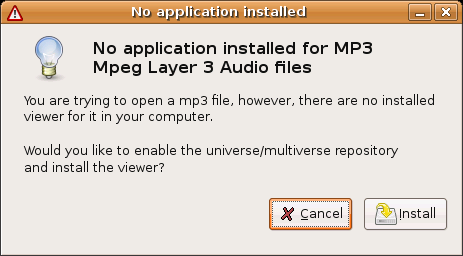
\includegraphics[scale=0.75]{figure/ubuntu_mp3.png}\label{dialog}
	\end{center}
	\caption{\textit{Il primo ``dialog'' per l'installazione del supporto MP3}}
\end{figure}

Questa soluzione, che a livello pratico non richiede particolari competenze informatiche come la capacità di installare il codec MP3 personalmente nel sistema, ha consentito ad Ubuntu di ottenere moltissimi utenti (soprattutto in Europa e negli stati ``liberi'') che non hanno sentito opprimente la copertura brevettuale di altri paesi arrivare fino al proprio.
% \section{Cosa si può fare/non fare in USA in questa circostanza}
% \section{Cosa si può fare/non fare in UE in questa circostanza}

%\include{capitolo5}
 \chapter{Conclusioni}

Con questo elaborato si è voluto differenziare nel primo capitolo i concetti di Proprietà Intellettuale e Industriale, che pur rimanendo molto simili, nascono da un sostrato abbastanza diverso, anche se rispettivamente la prima copre una serie di diritti maggiore della seconda, come riportato nella visione insiemistica in figura \ref{fig:PI} . I tipi di tutela quindi che derivano da entrambi sono leggermente diversi in quanto il primo si attaglia al diritto d'autore in generale e l'altro alla tutela dell'invenzione come prodotto industriale. Fatto questo si è passati a definire brevemente il concetto di copyright, dilungandosi invece leggermente nella descrizione dei brevetti e marchi, forme di tutela della Proprietà Intellettuale, in quanto più coerenti con la traccia della trattazione.

Il capitolo secondo si contraddistingue perché, dopo aver data la definizione di brevetto, entra nel merito di tutta la trattazione: la tutela del software attraverso lo strumento del brevetto. Su questo concetto emergono tutt'oggi pareri contrastanti, per questo motivo la trattazione si è fatta molto interessante. Si è percorso un breve excursus sulla tutela giuridica del software secondo copyright, successivamente si è riassunto la storia dei brevetti software in UE e in USA, dandone una visione dall'alto e riportando i casi giuridici principali di ogni paese.

La trattazione poi si è spostata su tempi più recenti e ambiti tecnici. In particolare nel capitolo terzo si è osservato il tagliente punto di vista della Free Software Foundation nei confronti dei software patens, legati anche ad altre tecnologie recenti di restrizione dei diritti degli utenti. Si è quindi analizzato i nuovi articoli che compongono la nuova licenza copyleft: la GNU General Public License versione 3.
Infine si è dato un esempio degli effetti provati da questa, nella distribuzione del software gplv3 con software house che hanno sottoscritto patents agreement con altre lampante in questo è il caso Novell-Microsoft e il passaggio di licenza del software di interoperabilità tra reti Samba.

Ricordando di dare una veste pratica oltre che legale, l'ultimo capitolo prende come esempio il brevetto del formato di compressione audio per antonomasia, cioè l'mp3: il brevetto non è unico, ma sono una serie di brevetti detenuti da molte società; è stato quindi effettuato un lungo lavoro per districarsi nella rete brevettuale che si è formata. Prendendo questo caso, si vuole mostrare quali sono gli effetti della brevettazione, della difficoltà legata alla eterogeneità delle varie legislazioni e degli effetti apportate al free software o a software house commerciali.

Dalla trattazione è quindi emerso che il software è giusto che venga tutelato dal diritto d'autore; è anche vero d'altro canto che non può essere concepito solo come una mera composizione logico-intellettuale, visto l'enorme commercio del mercato del software. E quindi in questo senso è giusto affermare che anche il software,pur rimanendo un bene immateriale diverso dall'hardware, è entrato nella schiera dei prodotti industriali a tutti gli effetti. Appurato questo è giusto chiedersi se è lecito lasciare il software sotto copyright o addirittura applicare la nozione di brevetto, concepita per prodotti fisici o processi industriali, anche agli algoritmi implementati. Oppure invece notando l'uso che poi ne viene fatto dalle software house, potrebbe essere possibile negare l'applicazione del brevetto al software, in maniera congrua con quanto affermato dalla Free Software Foundation nella GPLv3, magari trovando una via alternativa tra la tutela intellettuale troppo generica e la tutela industriale troppo legata al monopolio.



\appendix

%\include{appendici}

\backmatter
\bibliographystyle{IEEEtran}
\bibliography{bibliografia}
%\include{biblio}

%\printindex % se si fa l'indice analitico.

\end{document}
